\documentclass[10pt,a4paper,twocolumn]{article}
\usepackage[utf8]{inputenc}
\usepackage[english]{babel}
\usepackage{amsmath}
\usepackage{amsfonts}
\usepackage{amssymb}
\usepackage{hyperref}
\usepackage{graphicx}
\usepackage{subfig}
\author{Roman Kessler}
\title{Mimicing Face Pareidolia with Computer Vision}
\begin{document}
\maketitle

\begin{abstract}
Placeholder
\end{abstract}

\section{Introduction}

Face pareidolia is the phenomenon of seeing faces in other patterns, where actually no face is present. A famous example is the face on mars (Fig.~\ref{fig:faceonmars}). Similar examples are known to everyone, when looking at clouds and imagining faces.

However, there has been an interesting series of experiments showing, that when subjects imagined faces in random noise, the neuronal areas of face processing are more active when imagining faces than when not imagining faces in a probe image~\cite{zimmermann2019illusory}. However, the nature of the face perception in random noise is of debate. Do images, labelled as face by a subject, contain some physical properties that may drive face perception (\emph{bottom-up paredolia}). Or alternatively, is the task - the instruction to find faces - that strong, that the subject randomly "chooses" some images to contain faces (\emph{top-down pareidolia})? The answer is probably a combination of both effects, alongside with a variety of other effects.

The aim of this study is to find any physical correlate of a face in random noise. For this we used a deep convolutional neural network with a binary face-classifier.


\begin{figure}
    \centering
    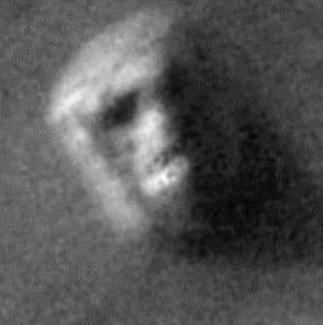
\includegraphics[width=3.0cm]{faceonmars.png}
    \caption{The \emph{face on mars} illusion \cite{carlotto1988digital}.}
    \label{fig:faceonmars}
\end{figure}

\section{Material \& Methods}

\subsection{Subject and data}

One subject was analyzed, which labeled 3295 random noise images with the extend of $43*32$px (Fig.~\ref{fig:stim}). The subject was convinced by a cover-story that around 50\% of images contain faces, which are barely visible. The appearing face should cover most part of the image. The subject has labeled 29\% of the images as face, and the rest as non-face.

\begin{figure}
    \centering
    
\includegraphics[width=3.0cm]{examplestim.png}
    \caption{Example stimulus. All stimuli consisted of random black and white pixels.}
    \label{fig:stim}
\end{figure}

\subsection{Binary face classifier}

To disentangle if there may be some physical correlate of a face in the stimuli, the subject labeled as "face", we constructed a binary face classifier. As a core network, we used the MobileNet architecture \cite{howard2017mobilenets}. We cut the fully connected layers at the end of the network, and replaced them by two fully connected layers, whereas the very last layer produced binary probabilities for two classes. We allowed the full model to be trained (no frozen layers).

\subsubsection{Training categories}

To create a binary face classifier we needed face and non-face training images. For the face-class, we randomly chose 8000 images from the \emph{ CelebFaces Attributes (CelebA)} dataset \cite{yang2015facial}, which contain faces of celebrities covering most part of the image area. For the non-face class, we chose 8000 cat and dog images from a public repository (\url{https://www.kaggle.com/chetankv/dogs-cats-image}).

\subsubsection{Training image preprocessing}

To train a model that shall later be tested on the noise images (Fig. \ref{fig:stim}), the images were first converted to greyscale, rescaled to $43x32$px, and lastly pseudo-converted to color because MobileNet expects 3 input channels (Fig.~\ref{fig:cat}).

\begin{figure}
    \centering
    \subfloat[][]{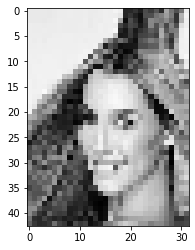
\includegraphics[width=3.0cm]{celeb.png}}
    \qquad
    \subfloat[][]{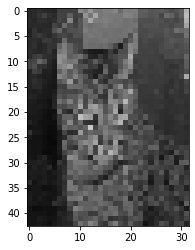
\includegraphics[width=3.0cm]{cat.png}}
    \caption{Example training images after rescaling. (a) First category were faces of celebrities. (b) Second category consisted of cat and dog stimuli.}
    \label{fig:train}
\end{figure}

\subsubsection{Training hyperparameters}

The training was conducted using Adam optimizer REF and categorical crossentropy as loss function. Only 5 epochs were repeated with batch size of 25 images. Already after 4 epochs, the training accuracy exceeded $0.99\%$, and cross-validation with a holdout dataset of 2000 images confirmed a less than $1\%$ error rate.

\subsection{Face classification in pure noise}

We then used the model to predict the classes of the random noise images (Fig.~\ref{fig:stim}). The prediction contains probabilities for both classes for each image, each summing up to~1. To test, if there is a difference (which we expected to be very tiny), we conducted a independent sample t-test on the probability of being categorized as face by the model. Therefore we split the probabilities according to the image labels, which were given by the subject.

\section{Results}




\section*{Data availability statement}

All used data, analysis pipelines, as well as further data of more subjects and further experiments can be retrieved from the GitHub repository of the first author \url{https://github.com/kesslerr/facepareidolia}.


\bibliographystyle{ieeetr}
\bibliography{Kessler2020pareidolia}

\section*{Supplementary Material}
\subsection*{MobileNet adaption}

\begin{verbatim}

model = Sequential()
model.add(MobileNet(weights='imagenet',include_top=False, input_shape = (43, 32, 3) )) 
model.add(Flatten())
model.add(Dense(100, activation='relu'))
model.add(Dropout(0.2))
model.add(Dense(2, activation='softmax')) # sigmoid

\end{verbatim}

\subsection*{}



\end{document}



